\section{ODE and Animation Practice}

The Lorentz System is chosen for this problem.

\begin{minted}{julia}
# Define a Lorentz System
function Lorentz_system!(du, u, p, t)
    # Unpack the system
    x, y, z = u
    σ, ρ, β = p

    # Dynamics
    dx = σ*(y - x)
    dy = x*(ρ - z) - y
    dz = x*y - β*z

    du[1] = dx; du[2] = dy; du[3] = dz
    return nothing # Absolutely nothing at all!
end
\end{minted}

\subsection{Implementation of Euler's Method}
An implementation of Euler's Method for solving ODEs is developed. This is defined as a single module as shown here.

\begin{minted}{julia}
module MySolvers

export ODESolution, Euler, euler_step!

# Define the solution data struct
struct ODESolution
    t::Vector{Float64}
    u::Vector{Vector{Float64}}
end

# Step wrapper (to prevent overpopulating the heap memory)
function euler_step!(system!, u, p, t, dt, du)
    system!(du, u, p, t)
    u .+= dt .* du
    return u
end

function Euler(
    system,
    initial_state::Vector{Float64},
    tspan::Tuple{Float64, Float64},
    parameters::Vector{Float64},
    delta_t::Float64
)
    t_start, t_stop = tspan
    number_of_steps = round(Int, (t_stop - t_start) / delta_t)

    t_vec = Vector{Float64}(undef, number_of_steps + 1)
    u_vec = Vector{Vector{Float64}}(undef, number_of_steps + 1)

    u_curr = copy(initial_state)
    du = similar(initial_state)
    t_curr = t_start

    t_vec[1] = t_curr
    u_vec[1] = copy(u_curr)

    for i in 1:number_of_steps
        euler_step!(system, u_curr, parameters, t_curr, delta_t, du)
        t_curr += delta_t

        t_vec[i + 1] = t_curr
        u_vec[i + 1] = copy(u_curr)
    end

    return ODESolution(t_vec, u_vec)
end
end # module
\end{minted}

\begin{figure}
    \centering
    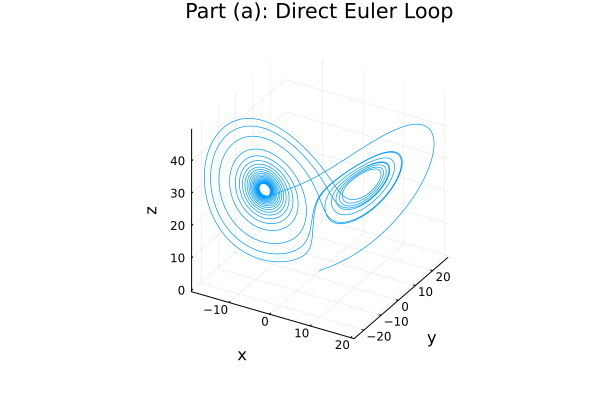
\includegraphics[width = 0.8 \textwidth]{Problems/Problem3/figures/lorenz_direct.png}
    \caption{Solution of the System using Euler's Method}
\end{figure}

\subsection{Estimating Accuracy}
One of the methods one can use to determine the accurracy of this implementation of Euler's Method is to compare its results to that of a higher order solver. For this purpose, the eigth-order solver \texttt{Vern8()} is used, with absolute and relative tolerances of $10^{-13}$.

In order to observe the change in accuracy of Euler's method, the time internal between consecutive integrations $dt$ is varied.

\begin{figure}
    \centering
    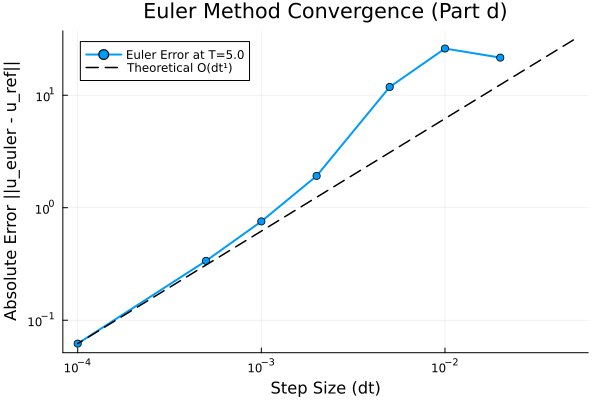
\includegraphics[width = 0.8 \textwidth]{Problems/Problem3/figures/euler_convergence.png}
\end{figure}

\subsubsection{Estimating Accuracy without Absolute References}
As shown in my Robotic Motion and Simulation report, one can estimate the accuracy of one's results using the Euler Method without an exact solution or high precision solver.


Estimating errors in numerical ODE solving (Euler's Method) and the relation so step size. This can be done without knowing the exact analytical solution. We know that

\begin{equation}
    x_{t+1}^{(h)} = x_t + h f(x_t, t),
\end{equation}

and thus

\begin{equation}
    x_{t+1}^{(h/2)} = x_t + \frac{h}{2} f(x_t, t).
\end{equation}

If we define the exact solution of the ODE to be $y_t$, and assuming that the error in Euler's Method is $\mathcal{O}(h)$, we may write that

\begin{equation}
    y_t = x_t^{(h)} + Ch + \mathcal{O}(h^2).
\end{equation}

With the difference

\begin{equation}
    x_t^{(h/2)} - x_t^{(h)} = \bigg(y_t - C\frac{h}{2} - \mathcal{O}(h^2)\bigg) - \bigg(y_t - Ch - \mathcal{O}(h^2)\bigg)
\end{equation}

and ignoring the $\mathcal{O}(h^2)$ term,

\begin{equation}
    x_t^{(h)} - x_t^{(h/2)} = C \frac{h}{2}.
\end{equation}

Thus, we may estimate the error $Ch = y_t - x_t^{(h)}$ as

\begin{equation}
    \text{error}(h) \approx 2 \bigg(x_t^{(h)} - x_t^{(h/2)} \bigg)
\end{equation}

\subsection{5thb Order Solvers (RK45)}
For a more pratical approach to numerically solving systems such as these, one may utilize 5th order solvers such as \texttt{RK45} or \texttt{Tsit5}.

\begin{figure}
    \centering
    \begin{subfigure}[b]{0.48\textwidth}
        \centering
        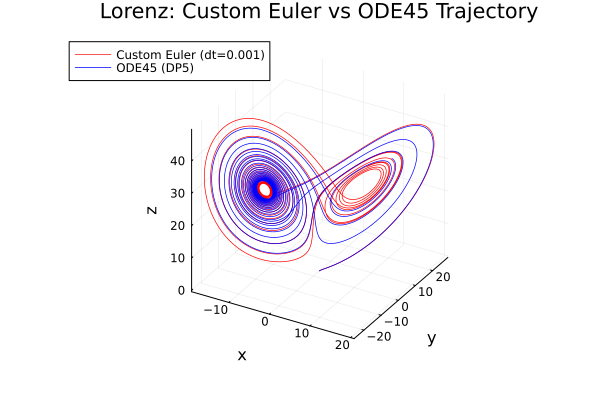
\includegraphics[width=\textwidth]{Problems/Problem3/figures/comparison_euler_vs_ode45_3d.png}
        \caption{Trajectory Comparision -- Euler's Method vs Tsit5}
    \end{subfigure}
    \hfill
    \begin{subfigure}[b]{0.48\textwidth}
        \centering
        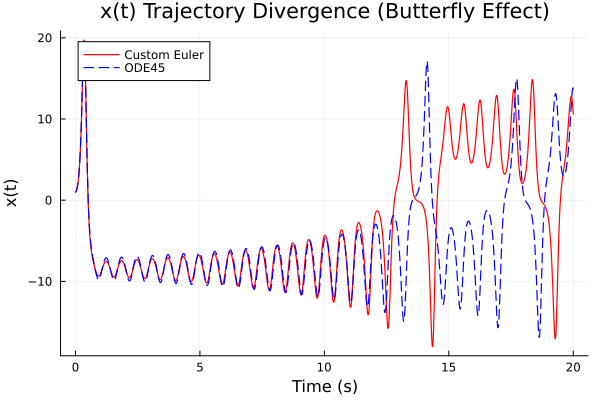
\includegraphics[width=\textwidth]{Problems/Problem3/figures/comparison_euler_vs_ode45_time.png}
        \caption{Trajectory Divergence -- -- Euler's Method vs Tsit5}
    \end{subfigure}
    \caption{5th Order Solution Results and Comparisons}
\end{figure}

\subsection{Error Estimation -- 5th Order Solvers}
A low-tolerance 8th order solver is used as a reference to compare \texttt{Tsit5} results to.

\begin{figure}
    \centering
    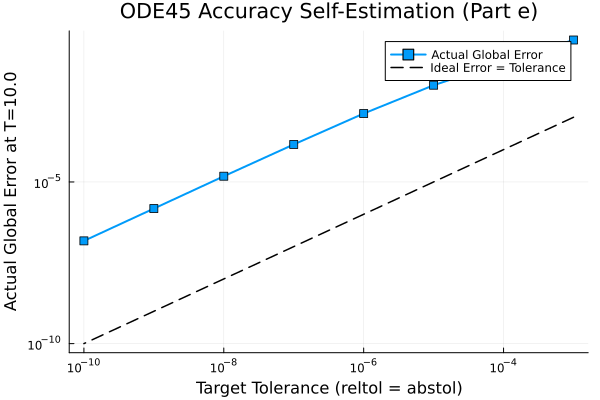
\includegraphics[width = 0.8 \textwidth]{Problems/Problem3/figures/ode45_accuracy_assessment.png}
\end{figure}

\begin{minted}{julia}
target_tols = 10.0 .^ (-3:-1:-10)
actual_errors = Float64[]

# High-precision ground truth at T = 10.0
T_tol_eval = 10.0
u_true_T = sol_ref(T_tol_eval)

for tol in target_tols
    sol_tol = solve(prob, DP5(), reltol=tol, abstol=tol)
    u_final_tol = sol_tol(T_tol_eval)
    push!(actual_errors, norm(u_final_tol - u_true_T))
end

# Tolerance Assessment Plot
plt_tol = plot(target_tols, actual_errors, xscale=:log10, yscale=:log10,
               marker=:square, lw=2, label="Actual Global Error",
               xlabel="Target Tolerance (reltol = abstol)", 
               ylabel="Actual Global Error at T=10.0",
               title="ODE45 Accuracy Self-Estimation (Part e)")

plot!(plt_tol, target_tols, target_tols, label="Ideal Error = Tolerance", 
      ls=:dash, color=:black, lw=1.5)
\end{minted}

Julia's \texttt{Tsit5()} solver does not (seem to) appear self-error estimation. This claim must be investigated.